\section{Case Study: Tool Protocol Validation}

To demonstrate practical applicability, we evaluate AOP on a simplified
tool invocation workflow representative of production agent-tool systems.
The case study focuses on protocol adjudication quality, not tool business
logic, and therefore isolates validation behavior from downstream execution.

\subsection{Scenario and Workflow}

In modern AI agent stacks, an invocation lifecycle often follows four steps:
\begin{enumerate}
\item The agent emits an invocation artifact.
\item A validator checks structural and policy-level conformance.
\item The tool runtime executes only if validation passes.
\item Outputs and evidence are persisted for replay and audit.
\end{enumerate}

In many deployments, step (2) is implemented as parse-only schema checks.
AOP augments this stage with fixture-aware and gate-aware adjudication.
\begin{figure}[t]
\centering
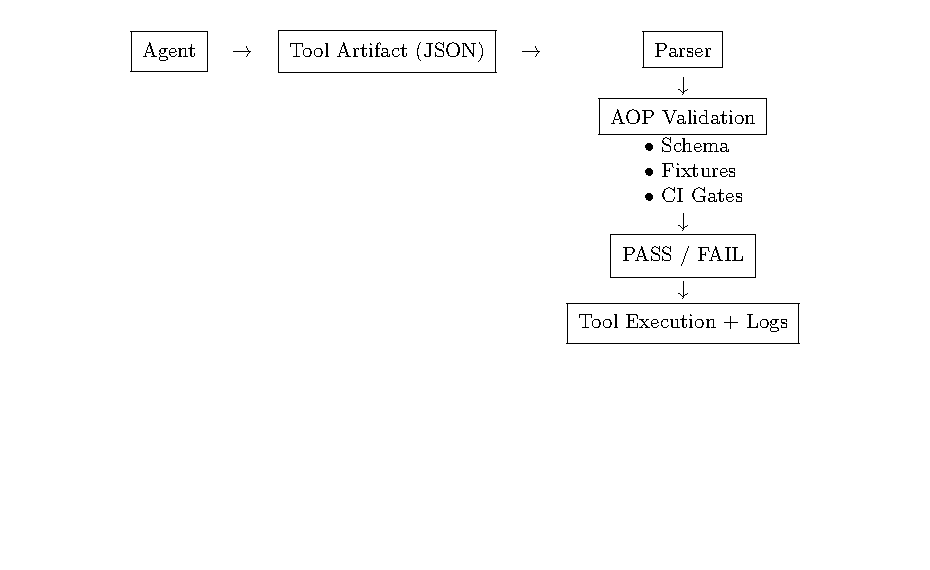
\includegraphics[width=0.9\linewidth]{figures/tool_protocol_flow.pdf}
\caption{Tool invocation workflow evaluated in the case study. Artifacts produced by AI agents are validated through AOP schema, fixtures, and CI adjudication gates.}
\label{fig:tool_protocol}
\end{figure}


\subsection{Concrete Protocol Instance}

To ground the case study in a concrete protocol shape, we use the
tool-invocation artifact below as a representative valid request:
\begin{quote}
\ttfamily
\{\\
\ \ "aop\_version": "1.0",\\
\ \ "kind": "tool\_invocation",\\
\ \ "id": "req-1042",\\
\ \ "tool": \{"name": "battery\_status",\\
\ \ \ \ "arguments": \{"asset\_id": "A-77"\}\},\\
\ \ "envelope": \{"payloadType":\\
\ \ \ \ "application/vnd.in-toto+json"\}\\
\}
\end{quote}

This artifact class is common in agent-tool ecosystems: a caller provides a
tool identifier, structured arguments, and an evidence envelope pointer.
Case-study invalid samples mutate this shape by removing required identity
fields, altering payload-type casing, or introducing unsafe numeric content.

\subsection{Artifacts and Data}

The case study uses the repository's executable artifact set, including
valid examples, negative fixtures, and adversarial invalid inputs.
The benchmark corpus size is 139 artifacts, and adversarial samples include
duplicate-key ambiguity, non-canonical in-toto payload type casing, and
unsafe integer edge values.

To keep the study reproducible, all checks are executed via scriptable
pipelines rather than manual inspection. This allows direct replay in CI
and local environments using identical commands and fixture directories.

\subsection{Baseline: Parse-Only Validation}

The baseline validator applies parse-level checks and schema loading without
semantic adjudication. This mirrors common minimal validation in real systems
where ``valid JSON'' is treated as sufficient precondition for execution.

In this setup, artifacts with semantic inconsistencies can still pass initial
validation if their syntax is accepted. Duplicate-key ambiguity is a canonical
example: permissive parsers often collapse repeated keys rather than rejecting
the artifact, creating non-portable interpretation risk across runtimes.

\subsection{AOP Validation Pipeline}

AOP validates artifacts through three deterministic layers:
\begin{itemize}
\item \textbf{Schema validation}: required fields, type constraints,
      and closed-world shape checks.
\item \textbf{Conformance fixtures}: positive and negative fixture outcomes
      encoded as executable expectations.
\item \textbf{CI adjudication gates}: automated PASS/FAIL gate decisions
      producing replayable logs.
\end{itemize}

An artifact must pass all layers to be admitted for execution.
If a gate fails, the artifact is rejected with explicit failure mode
classification (parse-stage or checks-stage), improving triage precision.

\subsection{Operational Results}

\begin{table}[t]
\centering
\caption{Case study outcomes on tool protocol artifacts.}
\begin{tabular}{lll}
\toprule
Stage & Metric & Outcome \\
\midrule
Baseline parse-only & Rejected artifacts & 0 / 139 \\
AOP determinism & Repeatability (3 runs) & identical \\
AOP adversarial gate & Rejected invalid cases & 3 / 3 \\
\bottomrule
\end{tabular}
\end{table}

The baseline confirms that parse-only acceptance is not an adjudication
criterion. Under AOP, repeated runs produce stable outputs, and adversarial
samples are deterministically rejected with no unexpected pass.

\subsection{Case Study Implications}

This case shows that protocol-by-artifacts is directly deployable in tool
invocation workflows without coupling to a specific runtime implementation.
The key operational gain is predictable gate behavior: teams can reason
about admissibility using replayable evidence instead of ad hoc parser
semantics.

The same structure can be extended to additional domains (policy decisions,
registry exchanges, and evidence envelopes) by adding fixture families and
gate checks while preserving the adjudication model.
